\section{
برنامه دامنه پروژه
}

\subsection{
نمودار
\lr{PC-WBS}
}

\begin{center}
  \begin{figure} [h!]
    { 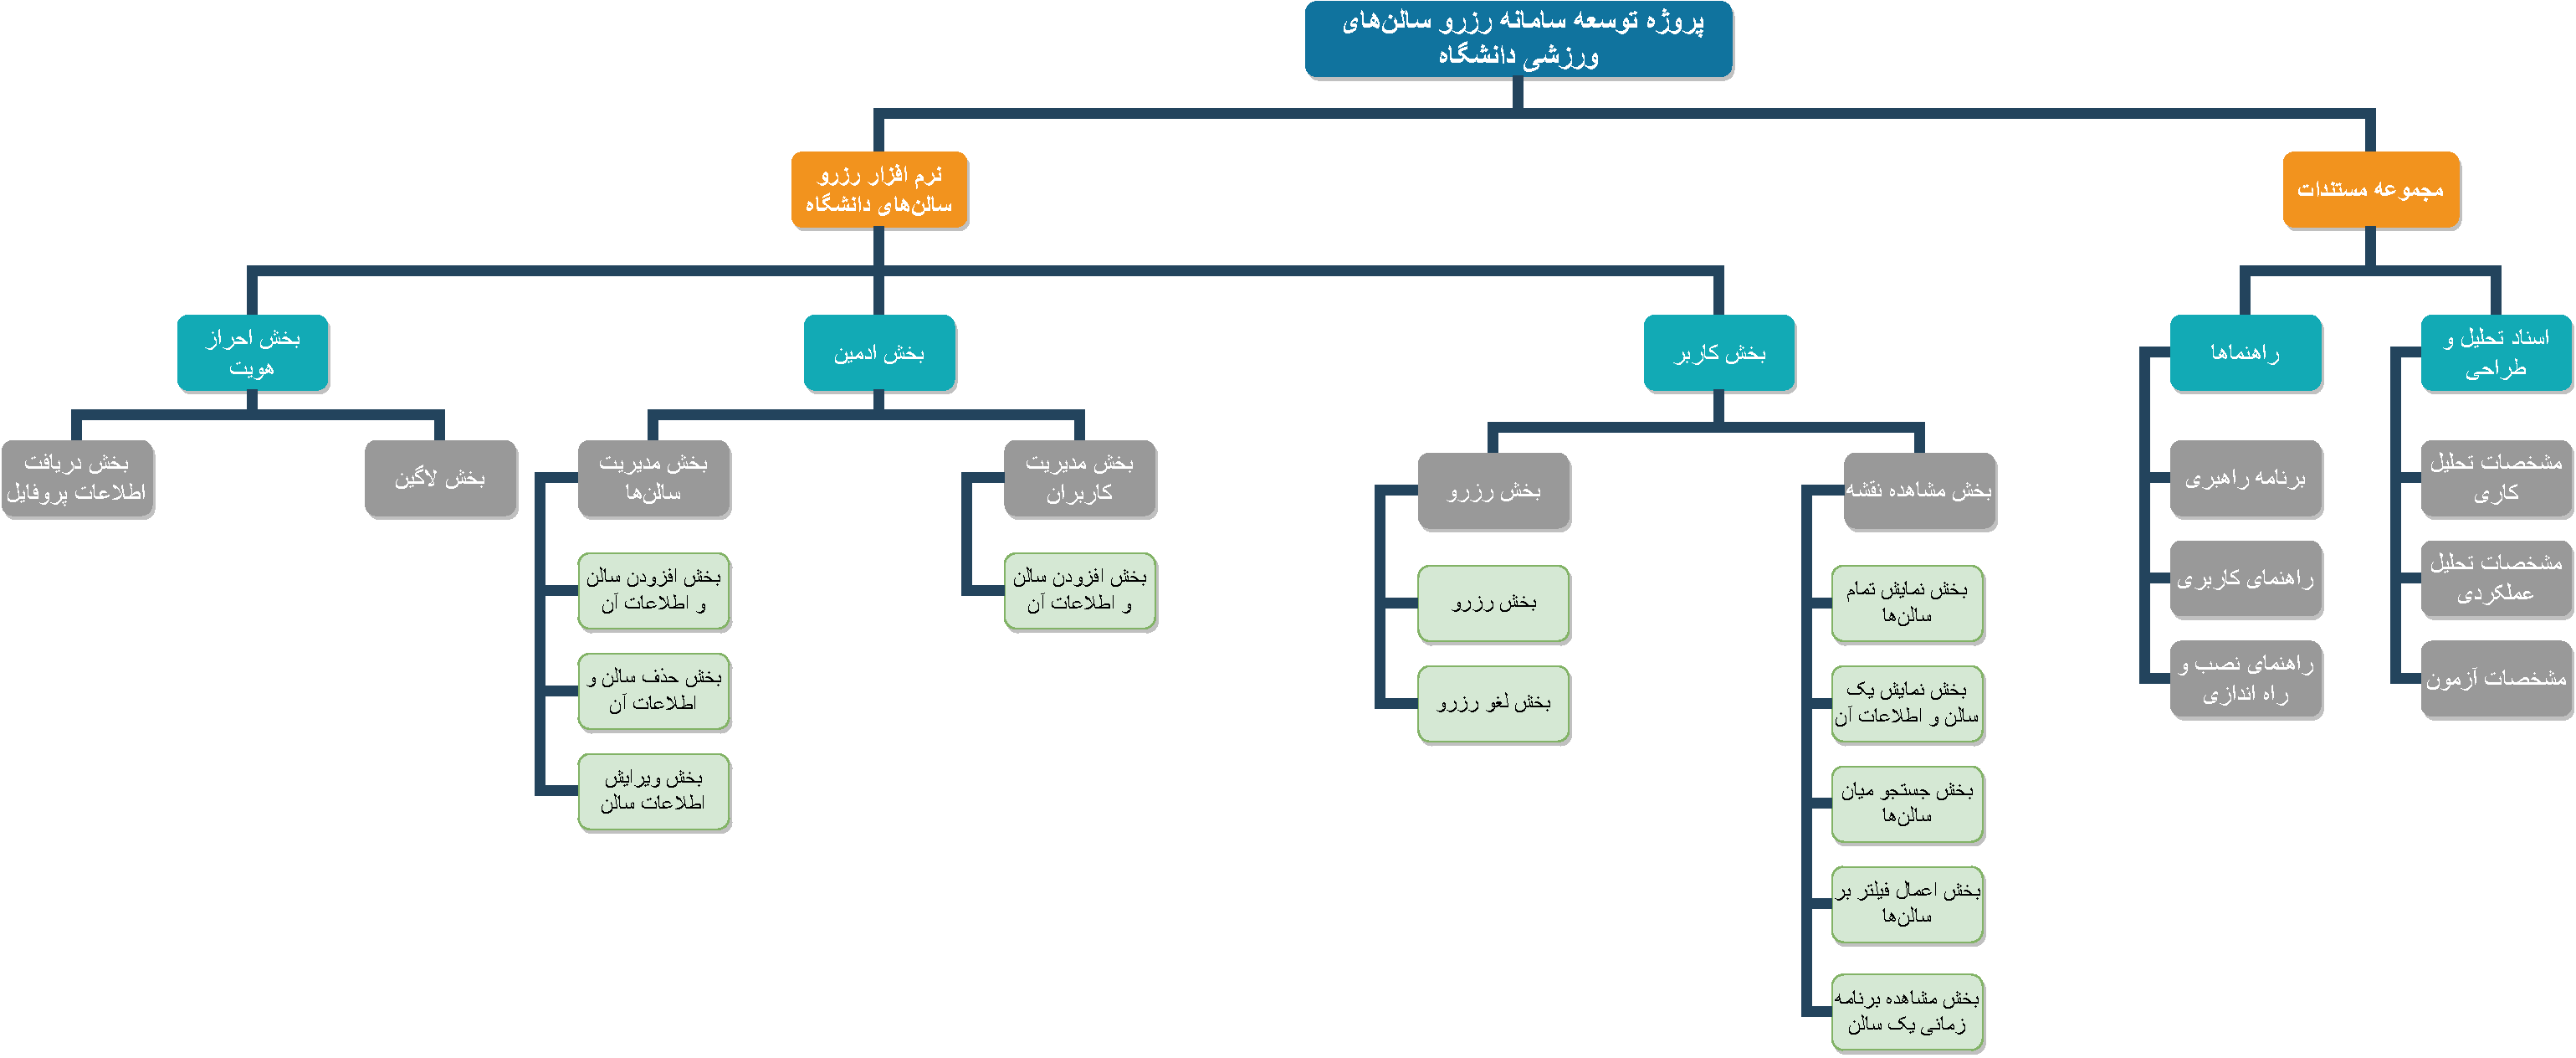
\includegraphics[page=1, width=\textwidth]{appandecies/PC-WBS.pdf}}
  \end{figure}
  \captionof{figure}[Short caption]{\lr{PC-WBS}}
\end{center}

\subsection{
نمودار
\lr{F-WBS}
}

\begin{center}
  \begin{figure} [h!]
    { 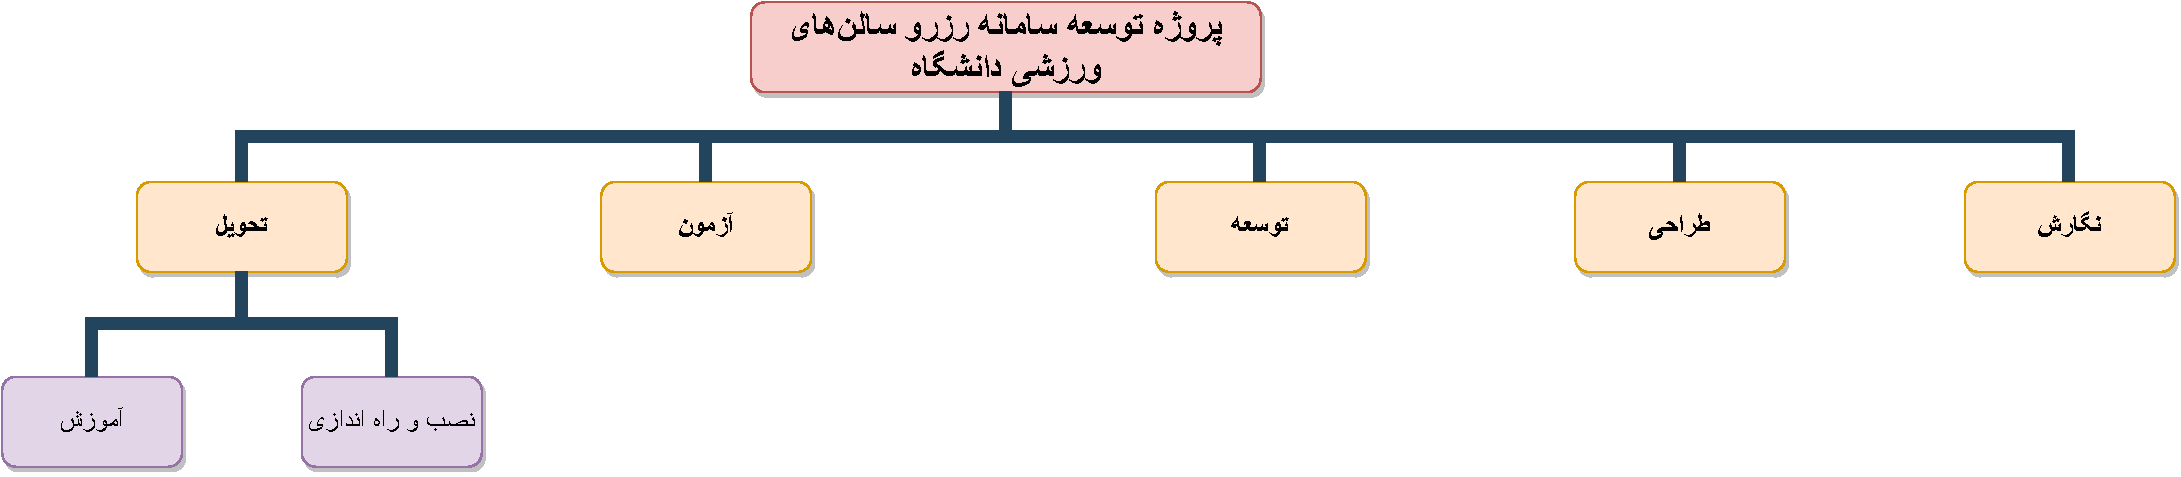
\includegraphics[page=1, width=\textwidth]{appandecies/F-WBS.pdf}}
  \end{figure}
  \captionof{figure}[Short caption]{\lr{F-WBS}}
\end{center}

\pagebreak
%\newpage

	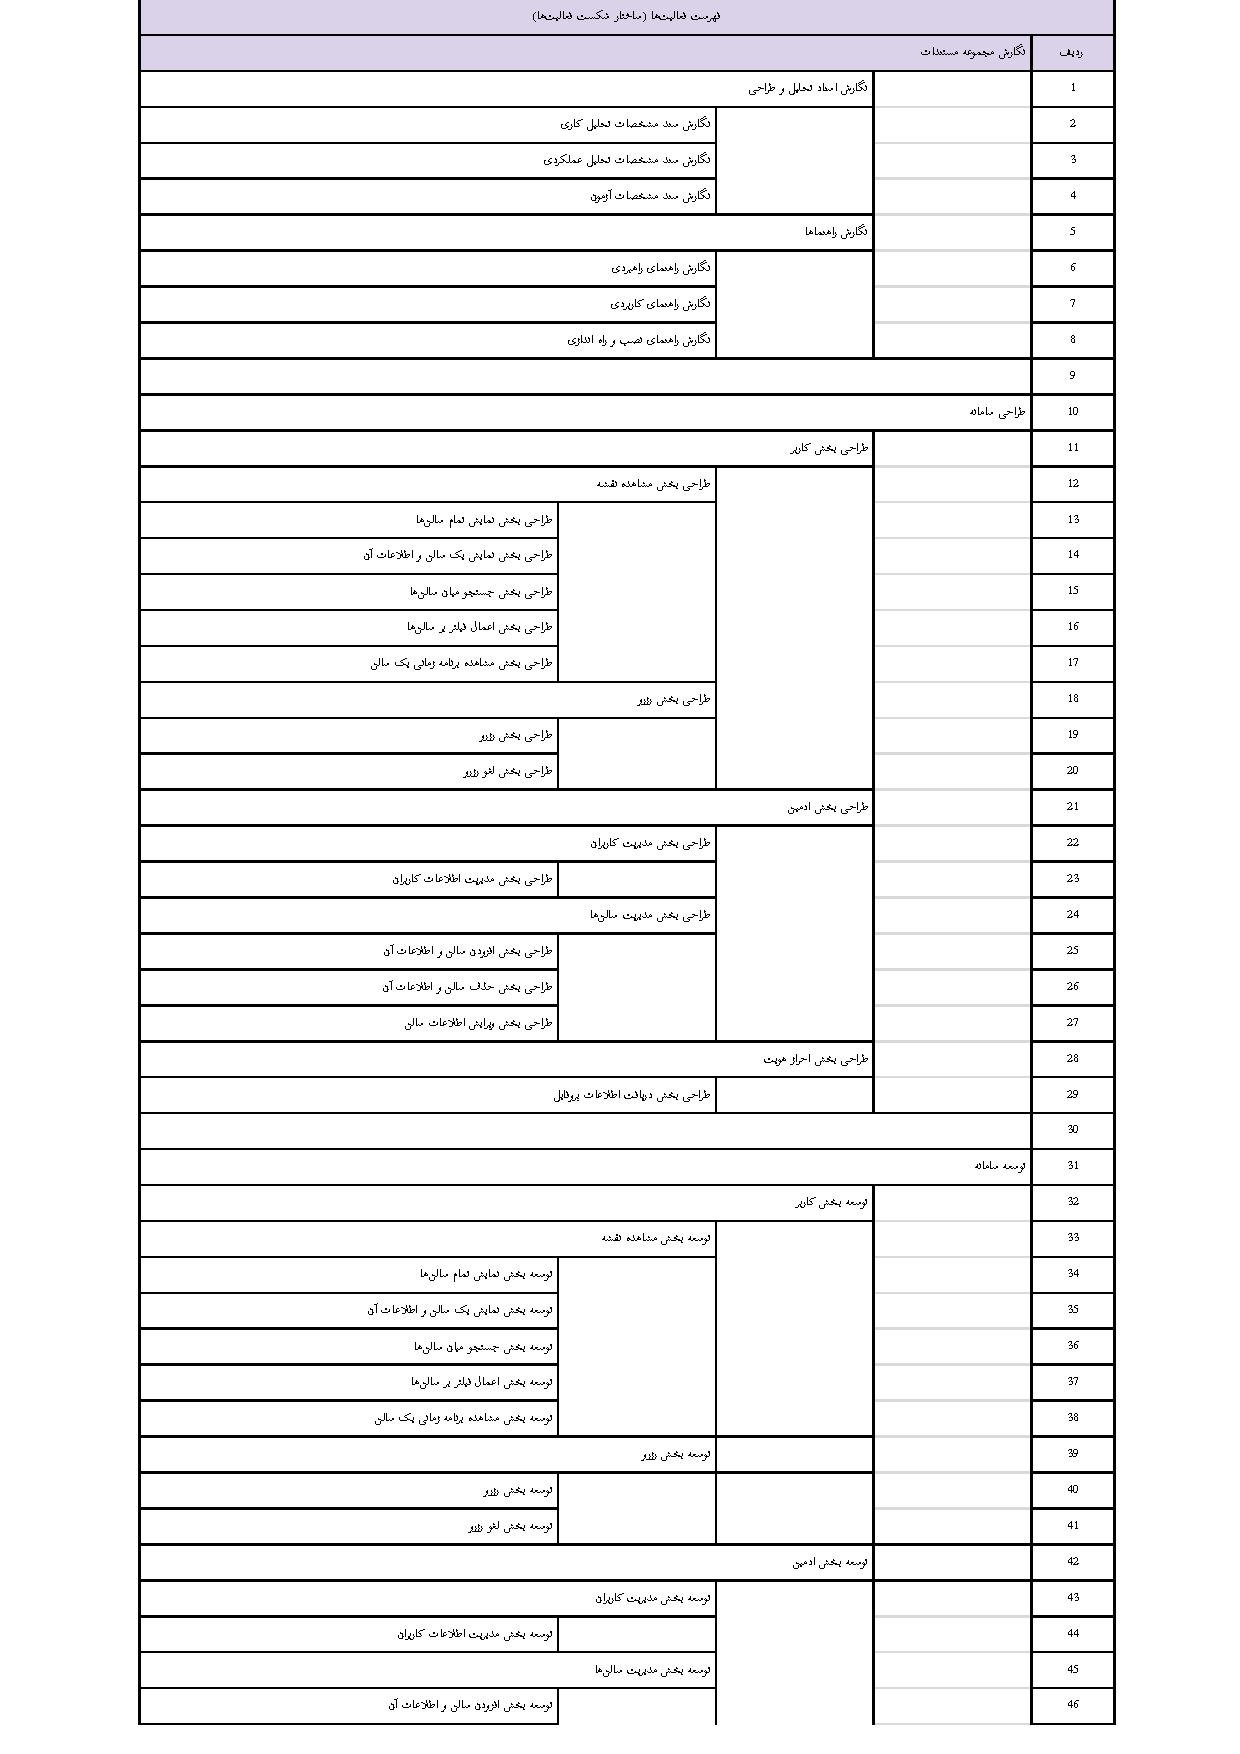
\includepdf[pages=-, width=\textwidth , scale = 1.5, pagecommand=\subsection*{\begin{flushright}
	\vspace{-0.5cm}
	\rl{
	فهرست فعالیت‌ها
	}
	\end{flushright}}]{appandecies/activity_list.pdf}
	\captionof{table}[Short caption]{ساختار شکست فعالیت‌ها}
%	\end{figure}
%\end{center}

\relax
%\begin{center}
%  \begin{figure} [h!]
%    { \includegraphics[page=2, width=\textwidth]{appandecies/activity_list.pdf}}
%  \end{figure}
%\end{center}



\subsection{
ماتریس ساختار شکست کار 
\lr{(Work Breakdown Structure)}
}

%\vspace{-0.5cm}
\begin{center}
  \begin{figure} [h!]
    { 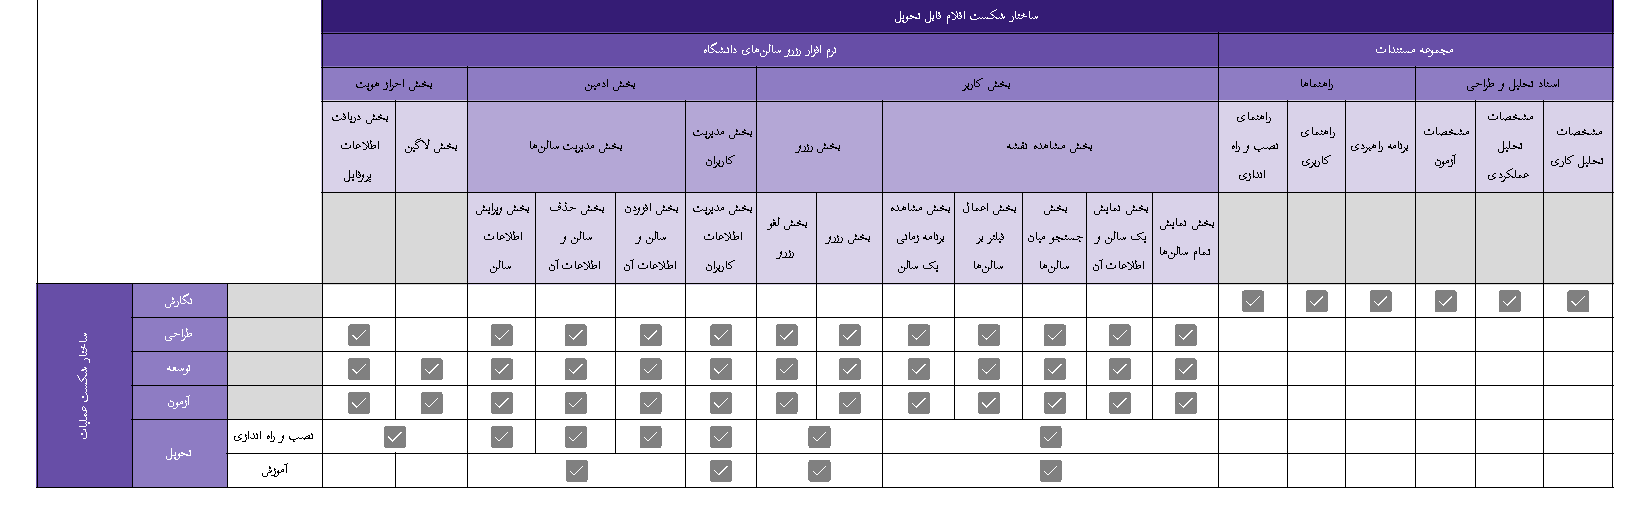
\includegraphics[page=1, width=\textwidth]{appandecies/WBS.pdf}}
  \end{figure}
  \captionof{table}[Short caption]{\lr{WBS Matrix}}
\end{center}